\newpage
\section{Evaluation}
\label{sec:auswertung}

All calculations and graphs were calculated using the \textit{python} package \textit{uncertainties}\cite{uncertainties}.
The captured data values for resistance, current and voltage have been assigned the uncertainties:
\begin{itemize}
    \item R[$\Omega$] $\pm\ 0.1$
    \item I[A] $\pm\ 0.0001$
    \item U[V] $\pm\ 0.01$
\end{itemize}

\subsection{Molar heat capacity at constant pressure}
During the execution of the experiment only resistances of the probe and shield and the current and voltage of the probe were monitored, see \autoref{tab:data}.
To calculate the molar heat capacity those values need to be transformed into temperature and energy.
With that the heat capacity can be calculated via \autoref{eq:heat_cap_v}.\\
\newline
To calculate the temperature of the copper probe, the following formula was provided in source\cite{V47}.
\begin{equation}
    T = 0.00134R^2+2.296R-243.02
\end{equation}
It gives the current temperature in C°, so in order to use it in calculations it needs to be transformed into units of Kelvin, by adding $273.15$.\\
The resulting temperature and its uncertainty is displayed in \autoref{fig:temp}.

\begin{figure}[H]
    \centering
    \subfloat[\centering]{{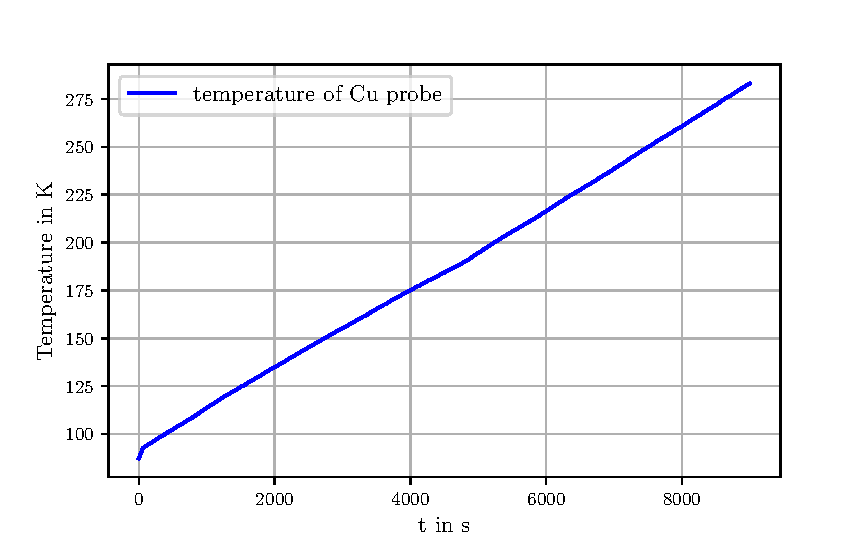
\includegraphics[width=12cm]{content/plots/temperature.pdf}}}%
    \qquad
    \subfloat[\centering]{{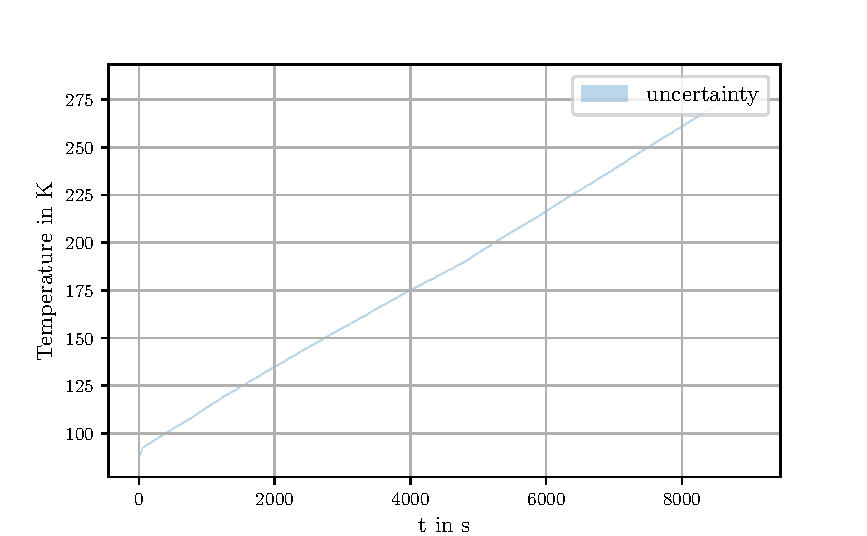
\includegraphics[width=12cm]{content/plots/utemperature.pdf}}}%
    \caption{a)The rise in temperature as time increases is linear and spans an interval between \SI{87}{\kelvin} and \SI{283}{\kelvin}.
    b)This graph shows the total area of uncertainty of the temperature graph in a). It is shown separately because the area is smaller than the temperature's line width.}
    \label{fig:temp}
\end{figure}

To use \autoref{eq:heat_cap_v}, the energy $E$ of the system must be calculated first, which is
\begin{equation}
    E = \Delta t \cdot P = \Delta t \cdot U \cdot I
\end{equation}
With the energy, the molar heat capacity at constant pressure follows \autoref{eq:cp}.
\begin{equation}
    C_P = \frac{E}{\Delta T}\cdot\frac{M}{m}
    \label{eq:cp}
\end{equation}
The additional term $\sfrac{M}{m}$ is included as the molar part, where $M$ is the molar mass of copper and $m$ the mass of the copper probe.
$\Delta T$ is the change in temperature.
The copper probe weighs \SI{342}{\gram} and the molar mass of copper is $M=$ \SI{63.546}{\gram\per\mol}\cite{copper}\\
\newline
Using \autoref{eq:cp} the resulting heat capacity $C_P$ averages to around \SI{23.75}{\joule\per{\kelvin\mol}} after approximately \SI{200}{\kelvin}, as seen in \autoref{fig:cp}.

\begin{figure}[H]
    \centering
    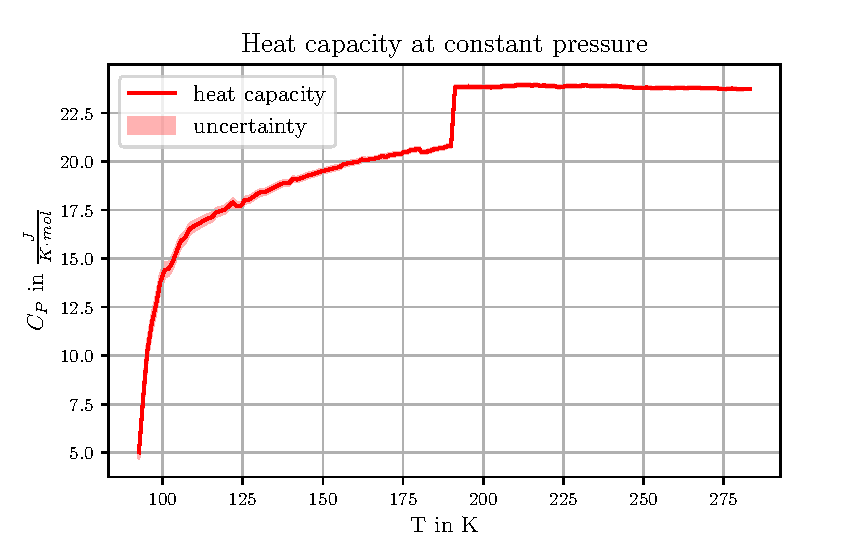
\includegraphics[]{content/plots/ucp.pdf}
    \caption{The molar heat capacity at constant pressure is displayed together with its uncertainty.}
    \label{fig:cp}
\end{figure}

\subsection{Molar heat capacity at constant volume}
As it is experimentally considerably easier to have a setup operate at a constant pressure, rather than constant volume, the molar heat capacity at constant volume can be calculated with a correction term based on the properties of copper.
The correction term states:
\begin{equation}
    C_V = C_P - 9\alpha^2\kappa V_0 T
    \label{eq:cv}
\end{equation}
Besides the temperature $T$, the other factors are the compression module $\kappa =$ \SI{137.8}{\giga\pascal}\cite{copper}, the molar volume $V_0 = 7.11\cdot 10^{-6}$ \si{\meter\cubed\per\mol}\cite{copper} and the thermal expansion coefficient $\alpha$.\\
The thermal expansion coefficient is described as linear in source \cite{V47} and a table with 24 values is provided.
Given that there are 150 measurements in \autoref{tab:data}, 24 values is not enough to assign a thermal expansion coefficient to every entry.
Therefore a fit was performed on the 24 given values based on a natural logarithmic function.\\
The resulting fit function is
\begin{equation}
    f(T) = 3.46524982\cdot \ln(T - 56.0189805) - 2.29906327
\end{equation}
\autoref{fig:expansion} shows the fitted function in comparison to the initial curve composed of 24 values.

\begin{figure}[H]
    \centering
    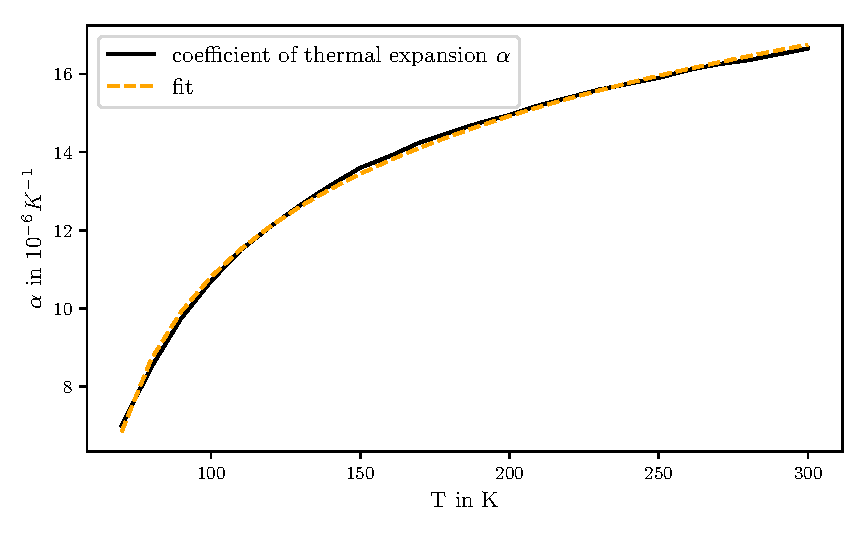
\includegraphics[]{content/plots/coefficient.pdf}
    \caption{This graph shows the thermal expansion coefficient given in source \cite{V47} for a temperature range of \SI{70}{\kelvin} to \SI{300}{\kelvin}, in comparison to the fitted function.}
    \label{fig:expansion}
\end{figure}

With the compression module $\kappa$, the molar volume $V_0$ and the thermal expansion coefficient known, the molar heat capacity at constant volume is calculated and shown in \autoref{fig:cv}.

\begin{figure}[H]
    \centering
    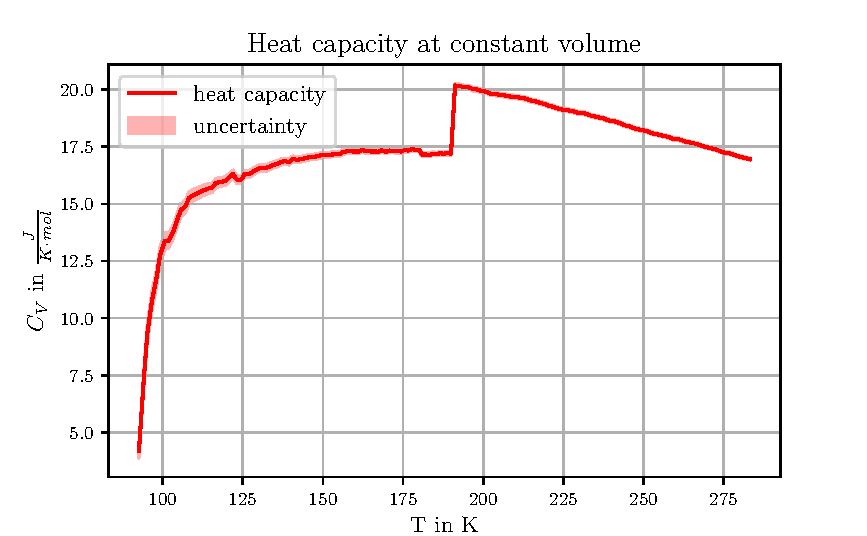
\includegraphics[]{content/plots/ucv.pdf}
    \caption{This graph shows the molar heat capacity at constant volume as well as its uncertainty against the temperature of the probe.}
    \label{fig:cv}
\end{figure}

\subsection{Debye temperature}
The Debye number $\frac{\theta_D}{T}$ is proportional to the molar volume heat capacity as seen in \autoref{eq:heat_debye}.
The table in source \cite{V47} provides a method of comparison by looking up the value of $C_V$ and assining it to a Debye number with an accuracy of $0.1$.
In this manner the Debye number has been determined and shown visually in \autoref{fig:debye}.

\begin{figure}[H]
    \centering
    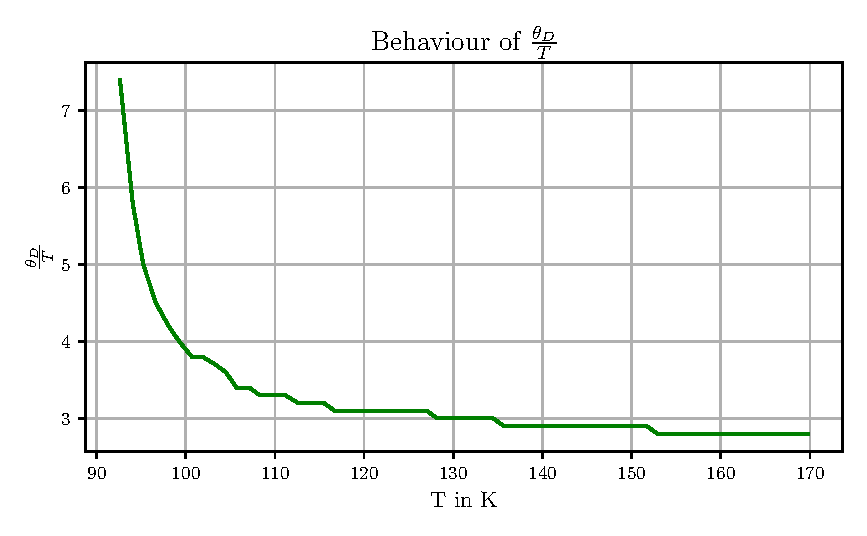
\includegraphics[]{content/plots/debye.pdf}
    \caption{This graph shows the Debye number at rising temperature in steps of $0.1$.}
    \label{fig:debye}
\end{figure}

The average Debye temperature from $T = 87\si{\kelvin} - 170\si{\kelvin}$ is $\theta_D \approx 415.425\si{\kelvin}$.
The average Debye temperature close to $T = 170\si{\kelvin}$ is $\theta_D \approx 443.113\si{\kelvin}$.

\subsubsection{Theoretical approach}
The Debye temperature can be calculated using the function
\begin{equation}
    \theta_D = \frac{\hbar\omega_D}{k_B}
    \label{eq:debye1}
\end{equation}
where $k_B$ in the Boltzmann constant and  $\omega_D$ is the Debye frequency.\\
The Debye frequency is dependent on the velocities of a transversal wave $v_{trans}$ and a longitudinal wave $v_{long}$ of copper.
\autoref{eq:debye2} shows the calculation formula for the frequency.
\begin{equation}
    \omega_D^3 = 18\pi^2 \frac{N_A}{V_0}\left(\frac{1}{v^3_{long}}+\frac{2}{v^3_{trans}}\right)^{-1}
    \label{eq:debye2}
\end{equation}
$N_A$ is the Avogardo constant and the velocities are given as $v_{trans} = \SI{2260}{\metre\per\second}$ and $v_{long} = \SI{4700}{\metre\per\second}$\cite{V47}.\\
\newline
The resulting theoretical Debye frequency is $\omega_D \approx 43.493\cdot 10^{12}\si{\per\second}$ and the Debye temperature $\theta_D \approx 332.208\si{\kelvin}$.